\documentclass{article}

\usepackage{amsmath}
\usepackage{amsfonts}
\usepackage{amssymb}
\usepackage{multicol}

\usepackage{mathenv}
\usepackage{multirow}

\usepackage{vmargin}
\setmarginsrb{2.5cm}{2.5cm}{2.5cm}{2.9cm}{0cm}{0cm}{0cm}{0cm}

\usepackage[utf8]{inputenc}

\usepackage[french]{babel}
\selectlanguage{french}

\usepackage{color}
\usepackage{hyperref}
\hypersetup{pdfborder={0 0 0}, colorlinks=true, urlcolor=blue, linkcolor = darkred}
\usepackage{graphicx}
\graphicspath{{fab/}, {ant/}} 
\usepackage{listings}
\definecolor{colKeys}{rgb}{0.75,0,0}
\definecolor{colIdentifier}{rgb}{0,0,0}
\definecolor{colComments}{rgb}{0.75,0.75,0}
\definecolor{colString}{rgb}{0,0,0.7}

\usepackage{verbatim}
\usepackage{moreverb}

\lstset{
basicstyle=\ttfamily\small, %
identifierstyle=\color{colIdentifier}, %
keywordstyle=\color{colKeys}, %
stringstyle=\color{colString}, %
commentstyle=\color{colComments}, %
showspaces=false,
}
\lstset{language=java}

% Commandes personnelles %

\definecolor{darkred}{rgb}{0.85,0,0}
\definecolor{darkblue}{rgb}{0,0,0.7}
\definecolor{darkgreen}{rgb}{0,0.6,0}
\definecolor{darko}{rgb}{0.93,0.43,0}
\definecolor{maintitle}{rgb}{0.66,0,0.22}
\definecolor{title}{rgb}{0,0.5,0.5}
\newcommand{\maintitlecolor}[1]{\textcolor{maintitle}{#1}}
\newcommand{\titre}[1]{\textcolor{title}{#1}}
\newcommand{\tsect}[1]{\titre{\section{#1}}}
\newcommand{\tssect}[1]{\titre{\subsection{#1}}}
\newcommand{\tsssect}[1]{\titre{\subsubsection{#1}}}
\newcommand{\vect}[1]{\overrightarrow{#1}}
\newcommand{\dred}[1]{\textcolor{darkred}{\textbf{#1}}}
\newcommand{\dgre}[1]{\textcolor{darkgreen}{\textbf{#1}}}
\newcommand{\dblu}[1]{\textcolor{darkblue}{\textbf{#1}}}
\newcommand{\dora}[1]{\textcolor{darko}{\textbf{#1}}}
\newcommand{\gre}[1]{\textcolor{darkgreen}{#1}}
\newcommand{\blu}[1]{\textcolor{darkblue}{#1}}
\newcommand{\ora}[1]{\textcolor{darko}{#1}}
\newcommand{\rouge}[1]{\textcolor{darkred}{#1}}
\newcommand{\ceil}[1]{\left\lceil #1 \right\rceil}
\newcommand{\cdil}[1]{\left\lfloor #1 \right\rfloor}
\newcommand{\term}[1]{\textit{\textcolor{maintitle}{#1}}}
\newcommand{\image}[1]{\includegraphics{#1}}
\newcommand{\imageR}[2]{\includegraphics[width=#2px]{#1}}
\newcommand{\imageRT}[2]{\includegraphics[height=#2px]{#1}}
\newcommand{\img}[1]{\begin{center}\includegraphics[width=400px]{#1}\end{center}}
\newcommand{\imag}[1]{\begin{center}\includegraphics{#1}\end{center}}
\newcommand{\imgR}[2]{\begin{center}\includegraphics[width=#2px]{#1}\end{center}}
\newcommand{\imgRT}[2]{\begin{center}\includegraphics[height=#2px]{#1}\end{center}}
\newcommand{\point}[2]{\item \ora{\underline{#1}} : \textit{#2}}
\newcommand{\bfp}[2]{\item \textbf{#1} : \textit{#2}}
\newcommand{\sumparam}[3]{\sideset{}{_{#1}^{#2}}\sum{#3}}
\newcommand{\sumin}[3]{\sideset{}{_{i=#1}^{#2}}\sum{#3}}
\newcommand{\sumkn}[3]{\sideset{}{_{k=#1}^{#2}}\sum{#3}}
\newcommand{\intin}[3]{\sideset{}{_{#1}^{#2}}\int{#3}}
\newcommand{\stitre}[1]{\noindent\textbf{\underline{#1}} \\}
\newcommand{\R}{\mathbb{R}}
\newcommand{\Z}{\mathbb{Z}}
\newcommand{\N}{\mathbb{N}}
\newcommand{\ualpha}{\vect{u_\alpha}}
\newcommand{\valpha}{\vect{v_\alpha}}
\newcommand{\palpha}{\vect{\Psi_\alpha}}
\newcommand{\npcomp}{\term{$\mathcal{NP}$-complet}}
\newcommand{\npcompl}{\term{$\mathcal{NP}$-complet} }
\DeclareMathAlphabet{\mathpzc}{OT1}{pzc}{m}{it}

\begin{sffamily}

\title{$ $\\ $ $\\ $ $\\ $ $\\ $ $\\ $ $\\ $ $\\\begin{Huge}\maintitlecolor{Gestion de projets logiciels}\end{Huge} \\ 
   $ $ \\ \begin{LARGE}\textit{Résumé blocus}\end{LARGE}}
\author{\textit{Xavier Dubuc} \\$ $ \\$ $ \\$ $\\ $ $\\ $ $\\ $ $\\ $ $\\ $ $\\ $ $\\ $ 
$ \\ 

\includegraphics{UMONS.jpg}}
%\date{}
\end{sffamily}

\begin{document}\begin{sffamily}

\maketitle

\newpage

\tableofcontents

\hbox{\raisebox{0.4em}{\vrule depth 0.4pt height 0.4pt width 10cm}}

\newpage

\section{Planification (PERT-GANTT)}

\subsection{Définitions}

\begin{itemize}
\item \textbf{Tableau d'étapes clés} : Date / étape clé $\rightarrow$ montre la liste des étapes clés du projet.
\item \textbf{Tableau de tâches} : DateDeb-DateFin / tâche $\rightarrow$ montre la liste des tâches du projet.
\item \textbf{Tableau d'allocation} : Tâche/personne/Durée(pers/jour)/Dépendances (Tâche(Etape clé)) $\rightarrow$ montre qui 
travaille sur quelle tâche et pendant combien de temps.
\item \textbf{Diagramme GANTT} : représente les relations temporelles entre les tâches (éventuellement décomposées en sous-
tâches), axe vertical = les tâches et axe horizontal = le temps. On représente souvent les étapes clés par des losanges.
\item \textbf{Diagramme PERT} : représente la dépendance entre les tâches afin de visualiser l'ordre partiel dans lequel les 
tâches doivent être réalisées. Il permet d'évaluer la durée de chaque tâche de manière péssimiste, réaliste et optimiste. Une
tâche = un noeud dans le graphe (rectangle) et une étape clé également (rectangle aux coins arrondis).
\item \textbf{Chemin critique} : chemin le plus long dans le graphe de tâche (diagramme PERT) c'est-à-dire le temps 
\textbf{minimum} pour mener à bien le projet.
\item \textbf{Temps lâche} \rouge{ST} \textit{(Slack Time)} : le temps maximum duquel on peut reporter la tâche concernée sans 
retarder le projet.
\item \textbf{Temps libre} \rouge{FF} \textit{(Free Float)} : le temps qu'une tâche peut prendre comme retard sans que ses 
successeurs encourent un retard.
\item \textbf{Date de début la plus tôt} \rouge{ES} \textit{Earliest Start} : faut-il vraiment expliquer ?
\item \textbf{Date de début la plus tard} \rouge{LS} \textit{Latest Start} : faut-il vraiment expliquer ?
\item \textbf{Date de fin la plus tôt} \rouge{EF} \textit{Earliest Finish} : faut-il vraiment expliquer ?
\item \textbf{Date de fin la plus tard} \rouge{LF} \textit{Latest Finish} : faut-il vraiment expliquer ?
\end{itemize}

\subsection{Analyse un diagramme PERT}

\subsubsection{Calcul des temps de début et de fin}

Il faut traverser le graphe en utilisant 2 règles :
\begin{itemize}
\item Quand un noeud est visité, on peut activer les noeuds qui sont accessibles par une transition à partir du noeud courant.
\item Avant de visiter un noeud $\rouge{n}$, tous les noeuds qui ont une transition vers $\rouge{n}$ doivent avoir été visités.
\end{itemize}

\begin{enumerate}
\item \rouge{\textbf{Traversée en avant}} : utilisée pour déterminer le(s) chemin(s) critique(s). Fonctionnement :
\begin{itemize}
\item Calculer les \textit{Earliest Start et Finish} de chaque tâche.
\item Commencer au noeud start et déterminer le temps total de chaque chemin jusqu'au noeud end.
\end{itemize}
\item \rouge{\textbf{Traversée en arrière}} : utilisée pour déterminer les \textbf{Slack Time}. Fonctionnement :
\begin{itemize}
\item Calculer les \textit{Latest Start et Finish} de chaque tâche.
\item Commencer par le noeud end et déterminer pour chaque tâche quand elle peut être commencée au plus tard tout en terminant 
le projet le plus tôt possible.
\end{itemize}
De manière plus simple : $$\boxed{ST = LS-ES}$$
\end{enumerate}

Dans ces graphes, un chemin critique est un chemin contenant des tâches qui ont des Slack Time $=0$. (chaque graphe sans étape-
clé en contient un) \\

Le \textit{Free Float} sera toujours inférieur au \textit{Slack Time}, il se peut également que ce \textit{Free Float} soit égal 
à 0 alors que la tâche ne se situe pas sur un chemin critique. Il est calculé en prenant le minimum des \textit{Earliest Start} 
de tous les successeurs d'une tâche $T$ et en y soustrayant le \textit{Earliest Finish} de la tâche $T$. Assez logiquement, une 
tâche $T$, qui finit au plus tôt en temps $t_{end} = 10$ et la tâche "successeur" de $T$ qui démarre le plus tôt démarre en 
$t_{deb} = 12$ ; implique que son $FF$ sera égal à 2 (vu qu'aucune autre tâche ne doit être commencée entre temps, sinon le 
minimum ne serait pas celui trouvé).\\

Si la tâche dépasse son \textit{Free Float}, \textbf{au moins} une de ses tâches "successeur" encourera un retard (celle de $ES$ 
minimum) et si cette tâche est sur un chemin critique, c'est \textbf{tout le projet} qui encourera un retard.

\newpage

\subsection{Traiter le retard}

\noindent \textbf{Comment détecter un retard ?} \\

\noindent 3 procédés sont donnés :
\begin{itemize}
\item \blu{Analyse de patinage (\textit{slippage})} en utilisant les lignes de glissade (\textit{slip lines}). Cela consiste 
à analyser les tâches qui sont en retard ou en avance sur l'horaire. On peut voir ces lignes de glissade sur un diagramme de 
GANTT. Pour rappel, une tâche est remplie par une couleur (ou autre) pour spécifier son avancement, il suffit dès lors de relier 
tous les points finaux de ces zones remplies (on part verticalement du haut du diagramme au jour de l'analyse, le jour courant 
normalement). Si la ligne est vers la gauche, c'est que la tâche est en retard sur l'horaire, si elle est vers la droite c'est 
qu'elle est en avance. \gre{Cette technique permet de gérer beaucoup de tâches en même temps} mais \rouge{pendant un seul moment 
dans le temps}.
\item \blu{Analyse des lignes de temps}. On représente les tâches par des lignes de haut en bas, elles représentent le temps 
planifiés pour ces tâches et on ajoute une boule au bout pour signifier que la tâche est terminée. On met sur l'axe vertical le 
temps actuel, on vérifie ainsi que les tâches sont bien terminées avant le jour qu'il était prévu. \gre{Cette technique permet 
de couvrir l'échelle de temps complète} mais \rouge{elle ne peut considérer que peu de tâches}.
\item \blu{\textit{Earned value analysys}}, on considère le temps que l'on a planifié comme le "budget du projet", le temps 
d'un tâche completée est crédité à ce budget.\\
\end{itemize}

\noindent \textbf{Comment récupérer d'un retard ?} \\

Cela exige la combinaison de différentes activités :
\begin{itemize}
\item Ajouter du personnel \textbf{experimenté} pour des tâches bien indiquées \textit{(en dehors du chemin critique)}.
\item Livrer le produit de manière \textbf{incrémentale} (trier les fonctionnalités, d'abord livrer la fonctionnalité 
importante, puis livrer les autres de manière incrémentale).
\item Replanifier l'horaire, en changeant la date butoire.
\end{itemize}

Il ne faut surtout pas supprimer des tâches essentielles (phases de test, verification et validation). Il ne faut également pas 
ajouter de personnes au projet car cela va le retarder encore plus \textit{(loi de Brooks)}. En effet, l'ajout de personne va 
apporter une hausse des communications à effectuer, si les personnes ne sont pas expérimentées il faut les former. De plus, 
certaines tâches ne peuvent être parallélisées .. par exemple, une femme enceinte doit attendre 9 mois, 2 femmes doivent 
attendre 9 mois aussi .. ! \\

\noindent \textbf{Comment traiter les retards ?} \\

Il ne faut pas être \textbf{optimiste}, le "tout se passera bien" n'est qu'utopie. On sous-estime bien souvent les problèmes de 
communication (avec le client, entre les membres de l'équipe, ...), l'imprécision et l'évolution des exigences, les problèmes 
techniques, ... $\Rightarrow$ loi de \textbf{Murphy} ! \\

Il ne faut pas sous-estimer le temps à consacrer aux tests, il faut prévoir plus de temps pour celle-ci que pour la phase 
d'implémentation. Réduire cette phase est une recette pour le désastre. Il faut faire de la vérification et de la validation 
tout au long du cycle de vie (analyse/conception/implémentation) et essayer de prévoir les erreurs avant qu'elles ne se 
produisent afin de les éviter et épargner le temps qui pourrait être perdu en résolvant ces erreurs.\\

Il faut également tenir à l'esprit qu'en corrigeant un bug on en crée souvent un autre. Pourquoi ? Et bien, en général le bug 
est difficile à cibler et il a des ramifications dans tout le programme. On corrige alors généralement les symptômes plutot que 
la cause... c'est souvent même un stagiaire ou autre qui corrige le programme et pas le créateur ! \\

Finalement, la loi de \textbf{Lehman} nous dit que plus un logiciel évolue plus le nombre de bugs augmente. De plus, les 
corrections apportées à ces bugs détruisent la structure du système et le rendent désordonné. Au final, le nombre de bugs 
explosent et détruisent la capacité d'évolution du logiciel. Il convient d'utiliser des méthodes de \textit{refactoring} pour 
éviter ce problème.

\newpage

\section{Modèles de processus}

Un \blu{modèle de processus de logiciel} est une approche générale pour organiser un projet en activités. C'est une 
représentation abstraite d'un processus de logiciel. Il aide le chef de projet et son équipe à décider quel travail devrait être 
effectué et dans quel ordre. Il s'agit d'une aide à la pensée et non une prescription rigide de comment faire les choses.\\

\noindent \textbf{\underline{Voici les différents modèles connus} :}
\begin{enumerate}
\item \blu{La cascade d'eau}.\\
\textit{Ce modèle suggère que les développeurs devraient suivre une séquence d'étapes bien définie. Il souligne également 
l'importance des exigences et de la conception.} \\
\textbf{\underline{Caractéristiques} :}
	\begin{itemize}
	\item une séparation \rouge{stricte} des étapes,
	\item le modèle inclut l'itération et la rétroaction (une boucle de rétroaction permet de modifier l'étape précédente),
	\item chaque étape est complétée par la documentation des accomplissements.
	\end{itemize}
\gre{\textbf{\underline{Avantages} :}}
	\begin{itemize}
	\item facile à gérer (facile à comprendre et à utiliser et les étapes-clés sont bien définies),
	\item facile à maintenir (à chaque étape les accomplissements sont bien documentés).
	\end{itemize}
\rouge{\textbf{\underline{Inconvénients} :}}
	\begin{itemize}
	\item la séparation des étapes est trop stricte et inflexible (on doit finir une étape avant de faire la suivante, les 
	étapes sont très artificielles, il est parfois difficile de déterminer la fin d'une étape)
	\item modèle approprié quand les exigences bien définies (difficile de changer les spécifications quand le processus est en 
	cours)
	\item aucune interaction avec le client (le client ne voit pas le produit avant la fin du projet, le client ne peut rien 
	utiliser tant que le produit n'est fait en entier, ... )
	\item le modèle implique qu'une fois le produit livré, il ne reste que de la maintenance à effectuer.
	\end{itemize}
	
\item \blu{Le modèle en V}.\\
\textit{Amélioration de la cascade d'eau, adresse explicitement l'assurance de la qualité. Avant de terminer chaque étape, une
étape de vérification doit être exécutée pour assurer la qualité. A la fin du processus, les résultats de chaque étape sont 
validés (en utilisant des tests).} \\
\gre{\textbf{\underline{Avantages} :}}
	\begin{itemize}
	\item Qualité assurée + idem que cascade d'eau j'imagine.
	\end{itemize}

\item \blu{Le modèle "livraison en phases"}.\\
\textit{Ce modèle présente la notion de développement incrémental. Après la spécification des exigences et la planification, le 
projet est divisé en phases, représentant chacune des sous-projets séparés. Ces phases sont déterminées de telle manière que 
chaque produit d'une phase peut être donné au client.}\\
Contrairement à la \blu{cascade d'eau}, certaines parties du système seront disponibles plus tot.\\
Comme la \blu{cascade d'eau}, toutes les exigences doivent être spécifiées avant que le developpement ne puisse commencer.

\item \blu{Le modèle "prototypage"}.\\
\textit{Un prototype est un modèle exécutable d'un système logiciel qui souligne des aspects spécifiques.}\\
\textbf{\underline{Caractéristiques} :}
	\begin{itemize}
	\item Un degré élevé de participation du client,
	\item une représentation tangible des exigences du client,
	\item très utile quand les exigences sont instables ou incertaines.
	\end{itemize}
2 types de prototypage :
	\begin{enumerate}
	\item \ora{Throw-away prototyping}, dans lequel l'objectif est de bien comprendre les exigences. Pour ce faire, les 
	prototypes sont utilisés très tot dans le développement pour clarifier les parties mal comprises. Une fois que les exigences 
	sont bien comprises, le prototype peut être jeté.
	\item \ora{Evolutionary prototyping} $\sim$ développement incrémental, raffinement des spécifications, des fonctionnalités 
	et de la performance par des prototypes successifs.
	\end{enumerate}
\gre{\textbf{\underline{Avantages} :}}
	\begin{itemize}
	\item Le client participe activement dans le développement du produit et reçoit des résultats tangibles rapidement. Ceci 
	mène au fait que le produit résultant est plus facile à utiliser et à apprendre.
	\item Applicable pour des systèmes interactifs de petite à moyenne taille ainsi que pour des parties de grands systèmes ou 
	encore pour des systèmes à courte vie.
	\end{itemize}
\rouge{\textbf{\underline{Inconvénients} :}}
	\begin{itemize}
	\item Manque de visibilité du processus,
	\item le produit développé n'est souvent pas de qualité commerciale (mal structuré, pas au norme de l'industrie),
	\item des qualifications spéciales peuvent être exigées des développeurs,
	\item des détails spécifiques peuvent être établis trop tôt (souvent à la demande de l'utilisateur).
	\end{itemize}
	
\item \blu{Le modèle "spiral"}.\\
\textit{Le processus est représenté par une spirale. Cette spirale est divisée par des régions de tâches (en général entre 3 et 
6). Ces tâches sont taillées selon les caractéristiques des activités du projet en cours. Chaque tour de la spirale (360 degrés) 
représente une phase du processus, chaque phase passe donc par toutes les régions du processus et chacune résulte en un 
prototype. On peut donc obtenir un raffinement du produit en parcourant plusieurs phases du processus.}\\

\begin{figure}[h!]
    \begin{center}
    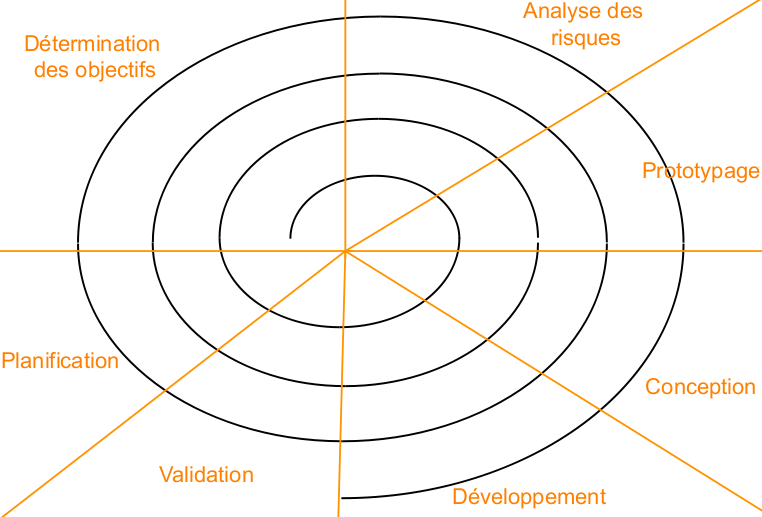
\includegraphics[width=200px]{img_001.png}
    \caption{Les régions de tâches}
    \end{center}	
\end{figure}

\gre{\textbf{\underline{Avantages} :}}
	\begin{itemize}
	\item plus réaliste et naturel que \blu{la cascade d'eau},
	\item conserve l'idée des phases mais l'intègre dans une approche itérative,
	\item le risque est un facteur pris en compte explicitement,
	\item le modèle peut utiliser une approche de prototypage.
	\end{itemize}
\rouge{\textbf{\underline{Inconvénients} :}}
	\begin{itemize}
	\item difficile d'apprendre le mode d'opération de ce modèle au client,
	\item l'évaluation des risques impose une expertise qui n'est pas du domaine des informaticiens.
	\end{itemize}

\item \blu{Le modèle de "développement formel"}.\\
\textbf{osef.}
\item \blu{Le modèle de "développement concourant"}.\\
\textbf{osef.}
\item \blu{Le modèle de "réutilisation des composants"}.\\
\textbf{osef.}
\item \blu{Le développement agile}.\\
\textit{Ensemble de principes et techniques légères pour répondre aux défis du développement moderne. On parle ici de :
\begin{itemize}
\item répondre à des problèmes complexes,
\item assurer des livraisons rapides,
\item atteindre le moindre coût,
\item faire face aux changements,
\item fournir un système de qualité.
\end{itemize}
Il s'agit d'une nouvelle approche au développement basé sur le développement et la livraison des incréments très petits de la 
fonctionnalité. \newpage Cette approche compte sur l'amélioration et l'évolution continue de code, le développement incrémental, 
la participation de l'utilisateur dans l'équipe de développement, la simplicité du processus et du logiciel ainsi que la 
vérification continue.}
\rouge{Cela fonctionne dans certains cas appropriés}, les systèmes ne doivent pas être critiques (au niveau sécurité) ni munis 
d'exigences volatiles.

Il y a différentes méthodologies agiles mais la plus importante est l'\textbf{extreme programming} :\\
\textbf{\underline{Caractéristiques} :}
	\begin{enumerate}
	\item Programmer par paires.
	\item Propriété collective du code.
	\item Développement \ora{dirigé par les tests} \textit{(test-driven development)} $\rightarrow$ aucun code ne peut être 
	rendu s'il n'a pas réussi tous les tests.
	\item Intégration continue.
	\item Cycle de livraison court (2 fois par mois par exemple).
	\item Refactoring pour réduire la complexité de la structure logicielle.
	\end{enumerate}
\textit{Le développement dirigé par les tests peut être utilisé comme micro-processus parmi les autres, il fonctionne comme sur 
le schéma ci-dessous.}
\begin{figure}[h!]
    \begin{center}
    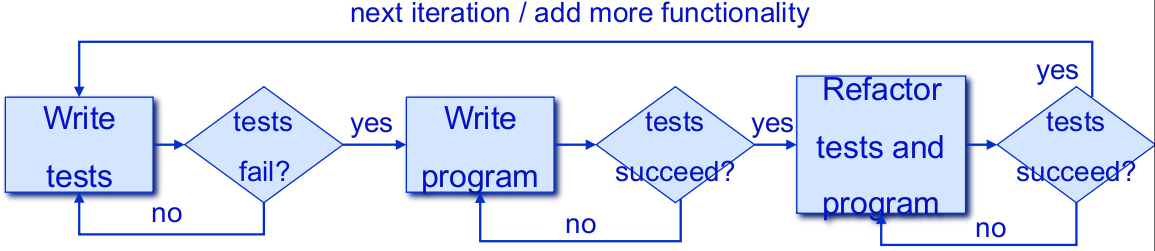
\includegraphics[width=250px]{img_002.png}
    \caption{Test-driven development}
    \end{center}	
\end{figure}

\rouge{\textbf{\underline{Inconvénients des développements agiles} :}} \\
\begin{itemize}
\item passage à l’échelle,
\item criticalité,
\item simplicité de conception,
\item rotation de personnel,
\item qualifications de personnel,
\end{itemize}

\end{enumerate}

\section{Validation et vérification}

Doivent être appliquée à chaque phase du projet.\\
\textbf{\underline{Différences} :} \\
\begin{itemize}
\item \rouge{Validation} : développer le produit correct, le logiciel doit se conformer au besoin réel de l'utilisateur.
\item \rouge{Vérification} : développer le produit \textit{correctement}, le logiciel doit se conformer à son cahier de charges 
et aux critères de qualité imposés (fiabilité, performance, ...).
\end{itemize}

\subsection{Vérification statique $\&$ dynamique}

\begin{enumerate}
\item \ora{Vérification statique} :
	\begin{itemize}
	\item \blu{inspections du logiciel} $\rightarrow$ analyse manuelle du logiciel pour découvrir des défauts, pour celà, un 
	cahier des charges précis doit être disponible, une équipe d'inspection connaissant les normes de l'organisation doit être 
	créée et le code ou les modèles syntaxiquement correct(s) doivent être disponibles.
	\item \blu{analyse statique} $\rightarrow$ analyse automatisée de la représentation statique du système pour découvrir des
	défauts comme des erreurs logiques, des anomalies dans le code (variable non initialisées par exemple) ou encore un manque
	de conformité par rapport aux normes et aux conventions. \\
	\textbf{\underline{Outils} : }PMD, FindBugs, Code Critics, Bad Smells, Lint, Lint++, Lint4j, JLint, CodeCheck, ...\\
	\textbf{\underline{Types} :}Analyse du flux de contrôle (boucles avec plusieurs sorties, code inatteignable...), analyse du 
	flux de données (variable utilisée avant initialisation, déclarée mais jamais utilisée, ...), analyse d'interfaces (mauvais 
	types de paramètres, ...) et analyse de pointeurs (pointeur null, ...).
	\end{itemize}
	\newpage
\item \ora{Vérification dynamique} :
	\begin{itemize}
	\item \blu{tester le logiciel} $\rightarrow$ concerné par exercer et observer le comportement du produit, s'assurer que le 
	logiciel contient le plus petit nombre d'erreurs, le système est exécuté avec des données de tests et son comportement 
	opérationnel est observé.
	\item \blu{analyse dynamique} qui peut être utilisée pour trouver des fuites de mémoire, vérifier la couverture du code et 
	analyser la performance.
	\end{itemize}
\end{enumerate}

\begin{center}
\begin{tabular}{rl}


\includegraphics[scale=0.05]{warn.png} & \rouge{Testing $\neq$ Debugging, le premier terme définit le fait d'établir qu'il y a} 
\\& \rouge{des défauts dans le programme, le second terme définit le fait de corriger ces 
défauts.}
\end{tabular}
\end{center}

L'analyse statique ne permet pas de découvrir tous les défauts, dès lors une analyse dynamique peut être plus qu'utile, surtout
pour un langage à typage dynamique.
\section{Gestion des risques}

Un \rouge{risque} est une probabilité qu'une certain circonstance défavorable se produise. \\
La \rouge{gestion des risques} est l'ensemble des activités reliées à l'analyse, l'évaluation et la mise en place de mesures 
destinées à comprendre et minimiser l'ampleur des risques informatiques. La gestion des risques est concernée par : 
\begin{itemize}
\item l'identification des risques qui peuvent affecter le projet,
\item la planification pour réduire l'ampleur des risques, pour qu'ils ne se développent pas en menaces principales.\\
\end{itemize}

\textbf{5 activités principales} :
\begin{enumerate}
\item \ora{Identification des risques}, voir sous-section suivante.
\item L'\ora{analyse des risques} consiste à évaluer le projet, la technologie et les ressources dans le but de déterminer et de 
comprendre la nature et l'origine des risques. Il faut déterminer la \rouge{sévérité} et la \rouge{probabilité} du risque. Le 
produit des 2 donne l'\rouge{importance} du risque.
\item La \ora{planification des risques} permet de décrire pour chaque risque identifié son importance par rapport au client, 
son importance par rapport au développement, les stratégies pour gérer ce risque et leurs implications économiques, le moyen de
vérifier que ce risque a été supprimé ou réduit et dans quelle mesure, les scénarios qu'il affecte ainsi que son allocation à un 
prototype. On utilise des stratégies pour ces risques :
\begin{itemize}
\item Stratégies pour éviter le risque $\rightarrow$ essayer de réduire la probabilité que le risque se produise.
\item Stratégies de minimisation $\rightarrow$ essayer de réduire l'impact du risque sur le projet ou le produit, quand il se 
produit.
\item Plans d'urgence $\rightarrow$ planifier comment traiter le risque, quand il se produit.
\end{itemize}
\item \ora{surveillance des risques} consiste à évaluer chaque risque régulièrement pour décider si sa probabilité ou ses 
conséquences négatives ont été modifiées.
\item \ora{traitement des risques}.
\end{enumerate}



\subsection{Types de risques}

\begin{itemize}
\item \textbf{Risques commerciaux} \\
La concurrence peut-elle capturer le marché avant que le produit ne soit prêt? Vaut-il mieux sortir une livraison minimale pour 
occuper le terrain?
\item \textbf{Risque financier} \\
L'entreprise dispose-t-elle de capacités financières suffisantes pour mener le projet à son terme?
\item \textbf{Risque technique} \\
La base technologique est-elle solide et éprouvée? 
\item \textbf{Risque de personnel} \\
L'équipe est-elle suffisamment expérimentée et maîtrise-t-elle les technologies mises en oeuvre?
\item \textbf{Risque de produit}, ils affectent la qualité ou la perfomance du produit. Par exemple, le programme ne tourne pas 
comme prévu;
\item \textbf{Risque d'entreprise}, ils affectent l'entreprise développant ou obtenant le logiciel.Par exemple, un produit de la 
concurrence sur le marché avant le notre, technologie utilisée dépassée, ... ;
\item \textbf{Risque de projet}, ils affectent l'horaire ou les ressources. Par exemple, le cahier des charges change plus que 
prévu.
\end{itemize}

\section{Gestion de la qualité}

Activités principales :
\begin{itemize}
\item \ora{planification de la qualité} consistant à identifier les caractéristiques de qualité à atteindre.
\item \ora{contrôle de la qualité} consistant à mesurer la qualité en utilisant des métriques.
\item \ora{assurance de la qualité} consistant à s'assurer que l'on atteint la qualité requise.
\end{itemize}

On utilise des \textbf{normes de qualité} pour pouvoir gérer la qualité, ces normes peuvent être définies au niveau 
internationale comme elles peuvent l'être au sein même d'un projet. Elles peuvent régir la qualité du produit comme la qualité
du processus.\\
\gre{Ces normes permettent une consolidation des bonnes pratiques (évite la reproduction de fautes déjà faites), 
offrent un \textit{framework} pour le processus d'assurance de la qualité et offrent également de la continuité dans le sens où 
de nouvelles personnes arrivant dans l'entreprise peuvent comprendre son fonctionnement en apprenant les normes utilisées par
celle-ci.}\\
\rouge{Elles ne sont cependant pas toujours appréciées par les développeurs (nécessité de les inclure dans le processus de 
normalisation de telle sorte qu'ils comprennent la raison impliquant l'utilisation d'une certaine norme). Ces normes sont
également difficiles à mettre à jour à cause du fait que la technologie évolue trop vite ; elles imposent également trop de
bureaucratie. Finalement, si elles ne sont pas supportées par des outils, elles demandent beaucoup trop de travail manuel.}

\subsection{Les métriques}

Utilisées pour mesurer la qualité d'un logiciel, on peut mesurer le nombre de lignes de code, le nombre de paramètres d'une 
méthode, ... Mais la meilleure façon (semble-t-il dire) est d'évaluer la \ora{complexité cyclomatique}. Cette complexité 
représente le nombre de chemin indépendants dans le graphe du flux de contrôle d'un programme, il s'agit également d'une limite
supérieure pour le nombre de tests nécessaires pour s'assurer que toutes les instructions ont été exécutées au moins une fois.

$$ \boxed{CC(G) = (\text{nombre d'arcs} - \text{nombre de noeuds}) + 2}$$
$$ \boxed{CC(G) = \text{nombre de noeuds de décision} + 1}$$

\subsection{!}

\begin{center}

\includegraphics[scale=0.05]{warn.png}
\end{center}

Je ne prétends pas que ce résumé est complet, donc si vous l'avez reçu (par je ne sais quel intermédiaire) dites vous que sans 
avoir lu les slides, ce résumé n'est sans doute pas suffisant ! \textit{(Je parle surtout pour certaines personnes/champix 
venant d'une contrée lointaine appellée Ville-Pommeroeul et répondant au joli nom de "Jean-Sébastien, la belette carnill'")}
\end{sffamily}\end{document}